\documentclass[a4paper,11pt] {article}
\usepackage{amsmath}
\usepackage[italian]{babel}
\usepackage{amsfonts}
\usepackage[utf8]{inputenc}

\pagestyle{empty}

\mag \magstep1
\oddsidemargin -1.0truecm
\textwidth 190truemm

\begin{document}

\begin{center}
\textbf{
Corso di Laurea in Matematica
\\
LABORATORIO DIDATTICO di MATEMATICA COMPUTAZIONALE
\\
a.a. 2017/18
\\
}
%--------------------------------
\line(1,0){150}
\end{center}

STUDENTE: Gori Davide
MATRICOLA: 550282
\begin{center}
	Esercizio sui Grafici
\end{center}

	Includiamo qui un grafico delle curve di Lissajoux ottenuto prendendo $x = sin(2t)$ e $y = cos(5t)$ con $t$ tra $0$ e $\pi$.
	
	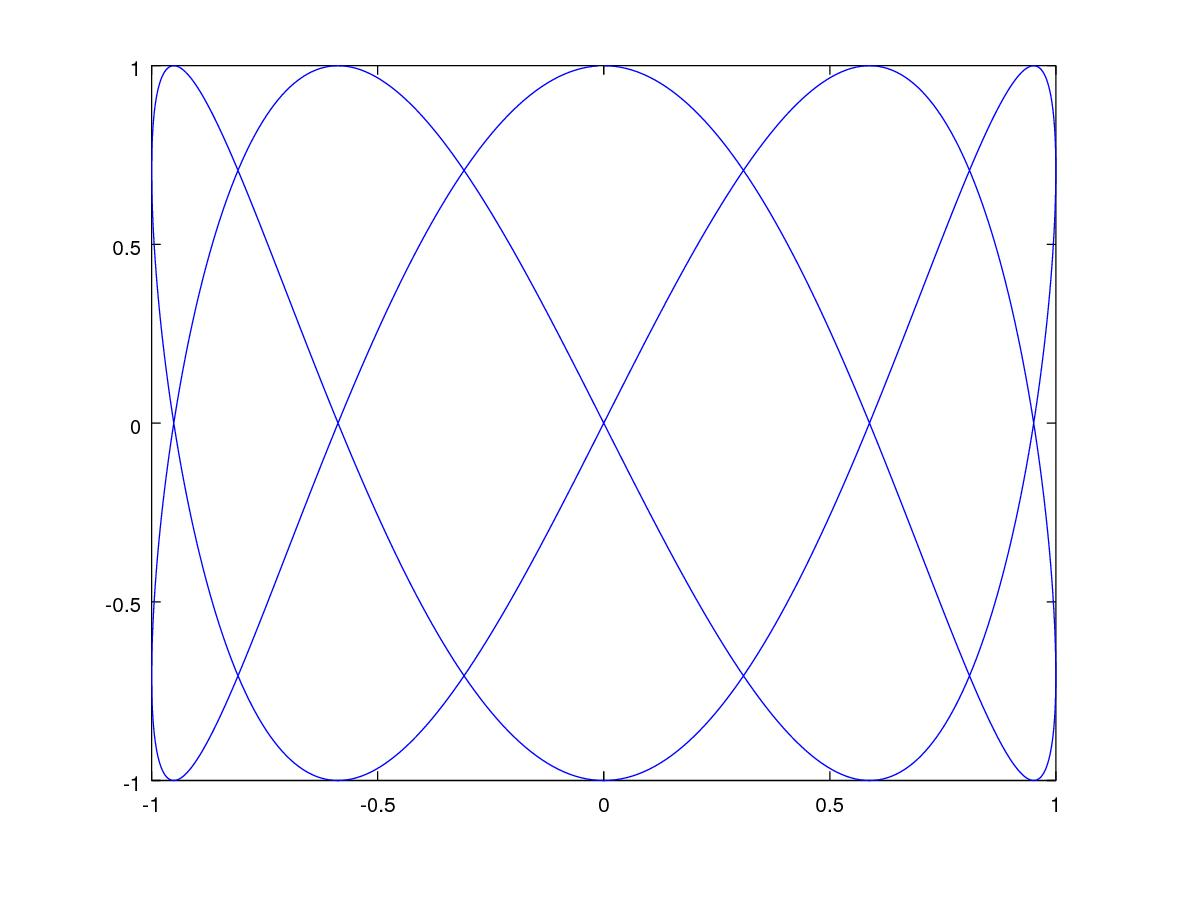
\includegraphics[width=\textwidth]{gra_1.jpeg}
	
	e poi un grafico tridimensionale della seguente funzione di due variabili $z=5 x^2-5 xy$ che mostra anche le linee di livello della funzione, rappresentata nel dominio $[-5, 5] \times [-5, 5]$.

	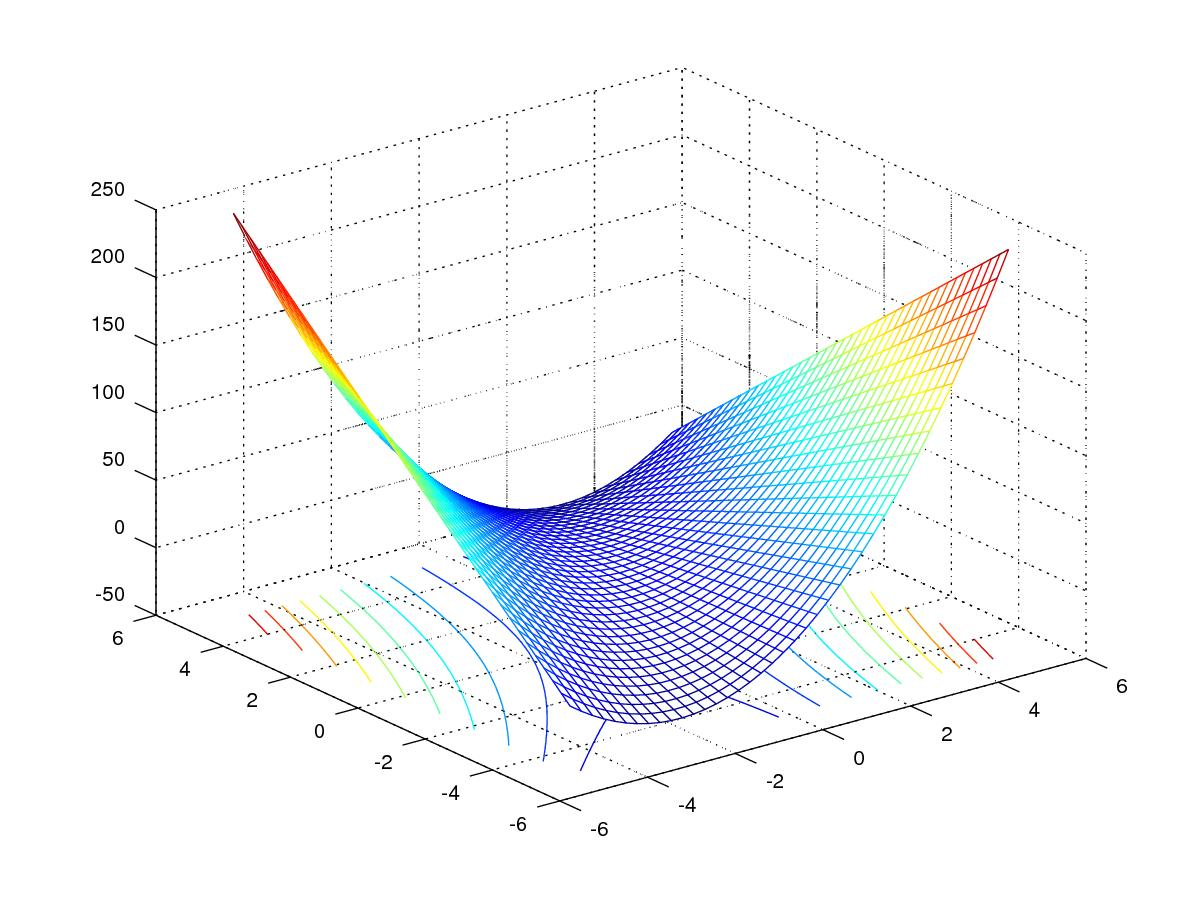
\includegraphics[width=\textwidth]{gra_2.jpeg}
	
	Pisa, 7 maggio 2018

\end{document}